\subsection{Introduction and plan of this chapter}

In this chapter we will present two NP-completeness results: for all
model extensions combined: bw + cv + fp + r, and for last three model
extensions: cv + fp + r. In the rest of this chapter we will name
first problem as model with bandwidth and second problem as model
without bandwidth. First observation that we do is that model with
bandwidth is a generalization of the model without bandwidth and
therefore we need to only prove NP-completeness of model without
bandwidth. However, the approach we chose is to first show the proof
for model with bandwidth, as it is simpler and shares its structure
with proof for model without bandwidth, therefore being good
introduction. Also, in this introduction we can write more about ideas
of construction, leaving technical lemmas for the final proof.

\subsection{NP-completeness of model with bandwidth}

We decided to make reduction from Boolean Satisfiability problem (SAT)
to our Virtual Cluster problem with bandwidth (VCB). SAT is decision
problem, but VCB is optimization problem with NO answer
possible. Therefore to make those problems compatible in terms of
reduction, we consider decision VCB variant, in which instance we have
additional constant $C$, and instance belongs to VCB if it has feasible
solution of cost $\leq C$.

Let's remind what decision VCB variant instance consists of:
\begin{enumerate}
\item constant $C$
\item balanced rooted tree $T$ with edge capacities $bw(e)$
\item constants $b_1$, $b_2$, which are costs of chunk transfer and
communication
\item constant $v$, which is desired number of VMs to be spawned
\item constant $ch$, which is number of types of chunks
\item sequence of chunks placed in leaves of $T$, possibly replicated
\end{enumerate}

Let's remind what SAT instance consists of:
\begin{enumerate}
\item clauses (let's name number of clauses as $cl(\Psi)$)
\item literals
\item variables (let's name number of variables as $var(\Psi)$
\end{enumerate}

Let's take any formula in Conjunctive Normal Form, name it $\Psi$ and produce
VCB instance $VCB_{\Psi}$. First, construct the tree $T_{\Psi}$. It will consist of
a root and separate gadget for each variable of $\Psi$, each of which
is a child of the root.


\begin{figure}[htbp]
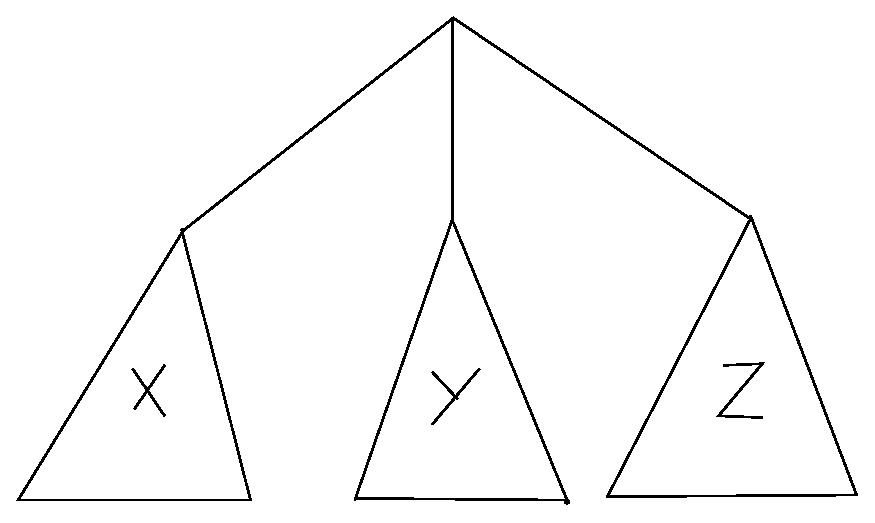
\includegraphics[width = \columnwidth]{figs/gadgets.eps}
\caption{Example gadgets for formula that contains variables x, y and z.}
\label{fig:gadgets}
\end{figure}

Gadget for variable $x$ has its root, $var(x)$, and two children:
$positive(x)$ and $negative(x)$. Vertex $positive(x)$ has $cl(\Psi)$
children: $x_1, x_2, \ldots, x_{cl(\Psi)}$. Vertex $negative(x)$ has
$cl(\Psi)$ children: $\neg x_1, \neg x_2, \dots, x_{cl(\Psi)}$. Every
gadget has the same structure: the same height, the same number of
leaves, and the same height. In fact, we will set bandwidth to be the
same everywhere in every gadget. Differences will be shown when we
will place data chunks.


\begin{figure}[htbp]
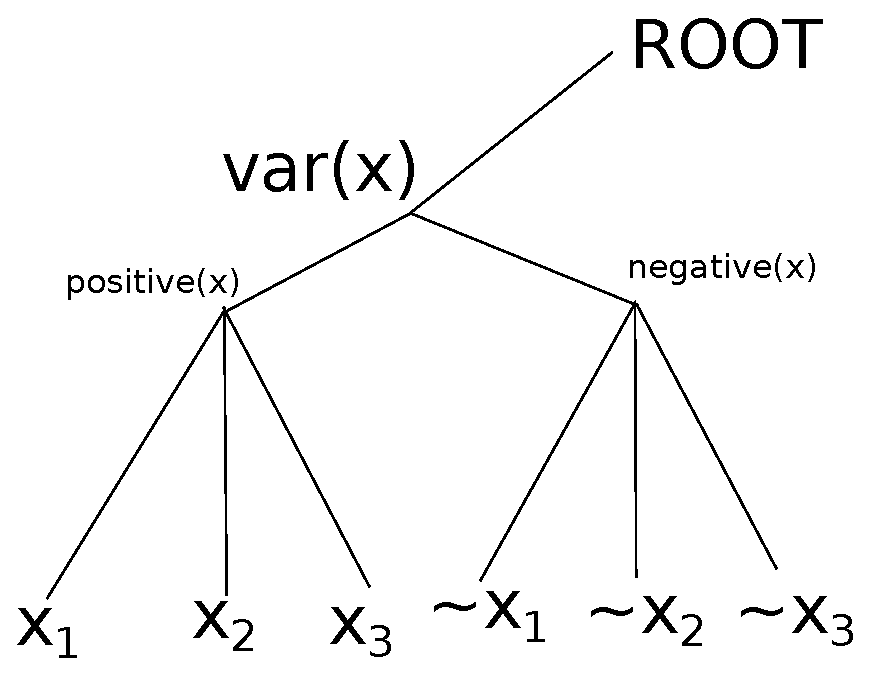
\includegraphics[width = \columnwidth]{figs/gadget-no-bw.eps}
\caption{Example gadget for variable $x$ in formula that has exactly
three clauses.}
\label{fig:gadgets}
\end{figure}

We set number of virtual machines to spawn to $v = cl(\Psi) \cdot var(\Psi)$.

Now we will set cost of chunk transportation and cost of communication
among virtual machines. We set communication cost to be $1$. We set
trasportation cost to be $b_1 = W$, where $W$ is constant large enough
to disallow transportation. It means that if virtual machine wants to
process the chunk, it has to be spawned where the data chunk is
placed. Technically, transportation is not completely disallowed, it
just inclines cost so huge that every optimal solution has no
trasportation.

Now we will set bandwidth constraints in $T_{\Psi}$. There are three
levels of edges in $T_{\Psi}$: top, middle and bottom. We set
bandwidth to unlimited at levels bottom and middle. At every edge of
top level, we set the same bandwidth to: $cl(\Psi) \cdot (var(\Psi) -
cl(\Psi))$. Idea behind capacity of this amount is that in every gadget we can
spawn at most $cl(\Psi)$ virtual machines. Let's prove it formally:

\begin{lemma} (bandwidth lemma)
Let $c$ and $v > 4$ be positive natural numbers. Let $a_1, a_2, \ldots,
a_v$ be natural number sequence that adds up to $c \cdot v$. Also, for
each $i$ we have $a_i \leq 2 \cdot c$. Then, if we have this:

$$ \forall_i a_i \cdot (c \cdot v - a_i) \leq c \cdot (c \cdot v -
c) $$

then each $a_i = c$.
\end{lemma}
\begin{proof}

Let's assume the contrary, which means that there exists such $y$ that
$a_y \neq c$. Then there are two cases: first, $a_y>c$ and second,
$a_y<c$. Proof for the first case is presented below; second case
with pidgeon hole principle results in existance of $a_z > c$, which
is basically the same (just substitute $a_y := a_z$ in proof below).

As we have $a_y < 2c$, we can say that $a_y$ has form $c +
k$ for $k \in [1, \ldots, c]$. Let's look at bandwidth inequality:

$$ (c + k) \cdot (c \cdot v - c - k) \leq c \cdot (c \cdot v - c) $$

After transforming it we have:

$$ 0 \leq k(k - (c \cdot (v - 2))) $$

Which is true for $k \leq 0$ or $k \geq c \cdot (v - 2)$, so no
positive $k \leq c$ can satisfy this inequality for $v > 4$, which gives a contradiction. 

\qed

\end{proof}

We will apply this lemma in following way. We interpret $a_i$ as
number of VMs that are spawned in $i$-th gadget. We set $c$ as number
of clauses and $v$ as number of variables. LHS of inequality from the
lemma is formula for communication cost of machines inside $i$-th
gadget to machines outside the gadget. RHS of the inequality is
bandwidth constraint for the gadget. Corollary from the lemma is that
any feasible solution must place exactly $c$ machines in every gadget.

TODO: We need to consider case where $v \leq 4$. First of all, it is
finite case, so we can do it by hand. We need to
produce an instance anyway though.

We set number of chunk types to be equal to number of clauses, $ch =
c(\Psi)$. To finish construction of $T_{\Psi}$, we need to place data chunks in
leaves. We do it the following way. For each clause of number $i$ we
construct as many replicas of chunk $c_i$ as there are literals in
clause $i$. For each literal $l$ (of form $v$ or $\neg v$) that satisfies clause $i$ we place
replica of chunk $c_i$ in leaf labeled $c_{l_i}$. TODO: draw example for
some simple formula.

To finish our construction, we need to set value of constant $C$. We
do it by calculating communication cost among spawned virtual machines in
certain solution to our instance. This soulution is constructed by placing
virtual machines in all leaves of $positive(v)$ and none in leaves
$negative(v)$ for every gadget for variable $v$. Please note that $C$
computed such way do not contain transportation cost. We will prove it
more formally in proof of model without bandwidth.

With our construction completed, we need to prove that it indeed
decides SAT.

\begin{theorem}Formula $\Psi$ is satisfiable iff $VCB_{\Psi}$ has
solution of cost $\leq C$.
\end{theorem}

\begin{proof}
($=>$) Let's take any valuation $F$ that satisfies $\Psi$. We will construct
solution to $VCB_{\Psi}$ using F in the following way. For each
variable $v \in var(\Psi)$ we place $cl(\Psi)$ virtual machines in
leaves of gadget $var(v)$. We need to choose $cl(\Psi)$ out of
$2 \cdot cl(\Psi)$ leaves to spawn VMs. If $F(v) = 1$, we spawn all VMs in leaves
of $positive(v)$, else we spawn all VMs in leaves of
$negative(v)$. Solution constructed such way has cost exactly
$C$, because VMs are evenly splitted among gadgets and VMs are not
mixed between $positive(v)$ and $negative(v)$ subtrees. We will prove
this claim in more detail in next proof. 

($<=$) Let's take any solution to $VCB_{\Psi}$ of cost $\leq C$. We
will construct valuation $F$ using placement of virtual machines in
solution to $VCB_{\Psi}$.

We need to take following observations. In every solution of cost
$\leq C$ every gadget has exactly $ch(\Psi)$ VMs spawned in its
leaves. It is true because we proved the bandwidth lemma. Also, inside
every gadget either all VMs are spawned in $positive(v)$ or all VMs
are spawned in $negative(v)$. It is true because cost of solution
where at least one gadget has VMs mixed between those branches is
always greater than $C$.

Now we can construct our valuation $F$. We do it the following way
(for each $v \in var(\Psi)$:

\begin{itemize}
\item if $v_1$ has machine in it then $F(v) = true$
\item otherwise $F(v) = false$
\end{itemize}

Valuation $F$ satisfies $\Psi$ because it satisfies every clauses, as
$VCB_{\Psi}$ solution processed all the chunks. No transportation of
chunks is allowed. Also, we have the property that if there is a VM in
$positive(v)$ subtree of any gadget, then:

\begin{enumerate}
\item every other leaf in $positive(v)$ has VM spawned in it
\item no leaf in $negative(v)$ has VM spawned in it
\end{enumerate}

\end{proof}

\subsection{NP-hardness of model without bandwidth}

There were only one use of bandwidth in proof from previous
chapter. It was to control number of VMs spawned in every gadget. For
model without bandwidth we need some other mechanism to control
it. Our high-level plan is like that:
\begin{enumerate}
\item Do not touch structure of previous proof.
\item Show new gadget for a variable.
\item Place new types of chunks in a tree.
\item Adjust number of VMs to spawn to work with new gadget.
\item Calculate new constant $C$.
\item Prove observations from previous proof. 
\end{enumerate}

Structure of construction is essentially untouched. We take any
formula $\Psi$ and construct instance of model without bandwidth,
$VC_{\Psi}$ that has solution of cost $\leq C$ iff $\Psi$ is
satisfiable. Our tree once again consists of gadgets for each
variable. Once again, we will have correspondence between clauses and
chunk types $c_1, c_2, c_{cl(\Psi)}$ (there are more chunk types in
construction though).

Let's start by presenting new gadget. Compared to the one from
previous proof, this one has one more level. Structure of the gadget
remains the same (we have $var(v), positive(v), negative(v), x_1,
x_2, \ldots, x_{cl(\Psi)}, \neg x_1, \neg x_2, \ldots,
x_{cl(\Psi)}$). Each of leaves labeled $v_i$ or $\neg v_i$ from previous gadget now is an inner
node and has two children; left of which is placeholder for variable chunk $c_{v_i}$ and
right is placeholder for chunks that correspond to clauses (like in
previous proof). We will label left child $l(v, i)$ and right child
$r(v, i)$. Please notice the use of replication: each variable
chunk appears exactly twice, once in $positive(v)$ and once in
$negative(v)$ (see figure).

\begin{figure}[htbp]
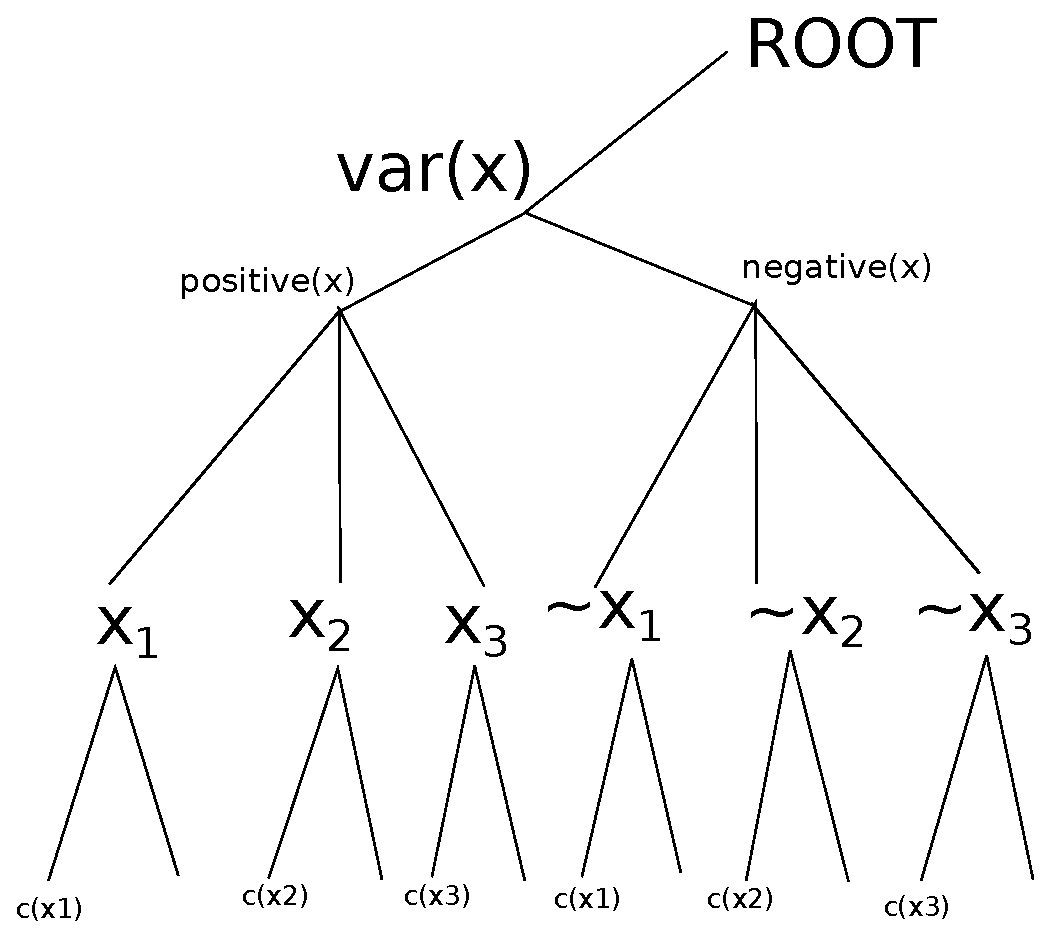
\includegraphics[width = \columnwidth]{figs/gadget-new.eps}
\caption{Example gadget for formula that contains exactly 3 clauses
and variable x.}
\label{fig:gadgets}
\end{figure}

This modification of a gadget introduces
$var(\Phi) \cdot cl(\Phi)$ new chunk types, so we need to double the number of VMs to
spawn: $v = 2 \cdot cl(\Phi)\cdot var(\Phi)$.


We calculate $C$ almost the same way as in previous proof. Once again,
we place VMs in $positive(v)$ and calculate communication cost
inclined. Let's calculate $C$ precisely this time. We split
communication cost into:
\begin{enumerate}
\item Communication among VMs placed in the same gadget. Number of VMs
placed in every gadget in our solution is $2\cdot cl(\Phi)$ and the
number of hops is $2$. Summing over every gadget gives:

$$ CC_1 = \sum_{i=1}^{var(\Psi)}2\cdot {cl(\Psi) \choose 2} $$

\item Communication among VMs placed in different gadgets. Number of
hops is $8$. Summing over every gadget gives:

$$ CC_2 = \sum_{i=1}^{var(\Psi)} 8 \cdot cl(\Psi) \cdot (cl(\Psi) \cdot (var(\Psi) - 1))$$
\end{enumerate}

$$ C = CC_1 + CC_2 = 2 \cdot var(\Psi) \cdot ({ cl(\Psi) \choose 2} +
4 \cdot cl(\Psi) ^2 \cdot (var(\Psi) - 1)) $$


We need to set transportation cost $b_1$. The idea is that cost of
transportation over even single hop is more costly than any possible
communication cost among $v$ VMs. Tree $T_{\Phi}$ has edge-height
equal to $4$, so we set $W$ to be sum of 8 hops communication among
all VMs:

$$ W = 8 \cdot {v \choose 2} $$

With our new construction completed, we need to prove that it indeed
decides SAT.

\begin{theorem}Formula $\Psi$ is satisfiable iff $VC_{\Psi}$ has
solution of cost $\leq C$.
\end{theorem}

\begin{proof}
($=>$)
Let's take any valuation $F$ that satisfies $\Psi$. We will construct
solution to $VC_{\Psi}$ using F in the following way. For each
variable $v \in var(\Psi)$ we place $2 \cdot cl(\Psi)$ virtual machines in
leaves of gadget $var(v)$. We need to choose $2\cdot cl(\Psi)$ out of
$4 \cdot cl(\Psi)$ leaves to spawn VMs. If $F(v) = 1$, we spawn all VMs in leaves
of $positive(v)$, else we spawn all VMs in leaves of
$negative(v)$.

Now we need to prove that our solution to $VC_{\Psi}$
has cost $\leq C$. First, we notice that communication among gadgets
(the $CC_2$) is the same as in calculation of $C$, because we put the
same amount of VMs in the gadgets. Second, we see that $CC_1$ is
exactly the same, because we put all the VMs on one side and therefore
number of hops is always $2$. TODO: find some way to refer to dummy
solution, name it, modify CC's to be parametrized by solution.

($<=$) Let's take any solution to $VCB_{\Psi}$ of cost $\leq C$. We
will construct valuation $F$ using placement of virtual machines in
solution to $VCB_{\Psi}$.

TODO:
\begin{enumerate}
\item Split further CC
\item Prove that in order to have solution of cost $\leq C$ all VMs in
r's have to be either on positive or in negative; do it by contradiction
\item Proove that in order to have solution of cost $\leq C$ all VMs
in l's have to be close to VMs in r's;
Do it by contradiction
\item Prove that there are exactly $2\cdot var(\Psi)$ VMs in every
gadget
\end{enumerate}

Now we can construct our valuation $F$. We do it the following way
(for each $v \in var(\Psi)$:

\begin{itemize}
\item if $v_1$ has machine in it then $F(v) = true$
\item otherwise $F(v) = false$
\end{itemize}

Valuation $F$ satisfies $\Psi$ because it satisfies every clauses, as
$VCB_{\Psi}$ solution processed all the chunks. Also, we have the
property that if there is a VM in $positive(v)$ subtree of any gadget,
then:
\begin{enumerate}
\item every other leaf in $positive(v)$ has VM spawned in it
\item no leaf in $negative(v)$ has VM spawned in it
\end{enumerate}


\end{proof}
